\section{Processi organizzativi}
\subsection{Gestione dei processi}
\subsubsection{Attività}
\paragraph{Gestione delle comunicazioni}
\subparagraph{Comunicazione interna}
Si utilizza Telegram\G\ per una comunicazione informale all'interno del 
gruppo, che inoltre fornisce il vantaggio di essere un'applicazione 
multi-piattaforma e disponibile anche in versione desktop/web. 

\subparagraph{Comunicazione esterna}
Il Project Manager\G\ sarà la persona preposta a mantenere i contatti con 
individui esterni al gruppo; per rappresentare il gruppo è stato creato il 
seguente indirizzo di posta elettronica:
\begin{center}
	starklabs.swe@gmail.com
\end{center}
Tutti i componenti del gruppo possono accedere alla casella, tuttavia solo 
il Project Manager\G\ si incaricherà di inviare le comunicazioni con questo 
indirizzo 
e-mail. 
Tutte le e-mail ricevute alla casella sopra indicata verranno automaticamente 
inoltrate ai membri del gruppo.

\subparagraph{Composizione email}
\begin{itemize}
\item \textbf{Destinatario:}
\begin{itemize}
\item \textbf{Esterno}: i destinatari possono essere il Proponente, Giulio 
	Paci e l'azienda Mivoq, il Prof. Tullio Vardanega o il Prof. Riccardo 
	Cardin.
\end{itemize}
\item \textbf{Mittente:}
\begin{itemize}
\item \textbf{Esterno:} l'unico indirizzo utilizzabile è 
	starklabs.swe@gmail.com e deve essere usato solamente dal Project Manager.
\end{itemize}

\item \textbf{Oggetto:} l'oggetto deve contenere [UNIPD-TTS\G] e dovranno essere indirizzate 
all'attenzione del referente Giulio Paci, così come è stato specificato nel 
capitolato dell'azienda Proponente. Nel caso il messaggio sia una risposta è 
necessario aggiungere la particella “Re:” all'inizio dell'oggetto per 
distinguere il livello di risposta; se si dovesse trattare di un inoltro si 
deve usare la particella “I:”. L'oggetto non va mai cambiato.

\item \textbf{Corpo:} in caso di risposta da parte dell'azienda Mivoq o del fornitore
risulta utile la citazione della frase a cui si intende rispondere. Il modello 
per citare correttamente deve seguire le seguenti regole. Devono essere 
presenti data e ora della mail a cui si risponde, il nome del mittente, il suo 
indirizzo e-mail tra parentesi angolari, ad esempio: <starklabs.swe@gmail.com>, 
la dicitura “ha scritto:” e infine il testo con una parentesi angolare chiusa 
prima, “>testo di prova”. Se dovessero essere presenti alcune parti con uno o 
più destinatari specifici, il nome dovrà essere indicato all'inizio del 
paragrafo tramite la dicitura: \textit{@destinatario}.

\item \textbf{Allegati:} qualora vi sia la necessità è data la possibilità di allegare alcuni file al 
messaggio e-mail. Possono essere usati per allegare il verbale di incontri con 
proponente e committente o i punti più importanti citati in una comunicazione 
Telegram\G.

\end{itemize}


\paragraph{Gestione delle riunioni}
\subparagraph{Riunioni interne}
\begin{itemize}
\item \textbf{Frequenza:} le riunioni del gruppo di lavoro avranno una frequenza settimanale; 

\item \textbf{Convocazione:} Il Responsabile di Progetto ha il compito di convocare le riunioni generali, a 
cui dovranno partecipare tutti i membri del gruppo.
Su decisione del Responsabile di Progetto le riunioni possono coinvolgere anche 
solo specifici componenti del gruppo, a seconda del ruolo che si ritiene più 
utile in una data fase del progetto. Al termine di ogni riunione viene redatto 
un verbale.
Il responsabile deve convocare l'assemblea, con almeno un giorno di preavviso, 
attraverso l'invio di una mail a starklabs.swe@gmail.com contente:
\begin{itemize}
\item \textbf{Oggetto}: convocazione riunione n. X, dove X indica il numero 
crescente di 
riunioni effettuate.
\item \textbf{Corpo}: 
\begin{itemize}
	\item \textbf{Data}: data e ora prevista;
	\item \textbf{Luogo}: luogo previsto;
	\item \textbf{Tipo}: ordinaria/straordinaria;
	\item \textbf{Ordine del giorno}: elenco numerato delle voci da esaminare.
\end{itemize}
\end{itemize}

Ogni componente del gruppo deve rispondere al messaggio in modo più celere 
possibile, confermando la presenza o giustificando un'eventuale assenza. Il 
Responsabile di Progetto, in mancata risposta di uno o più membri nel tempo 
utile, ha il compito di contattarli telefonicamente. Una volta ricevute le 
risposte e verificata l'assenza o presenza dei membri richiesti, il 
Responsabile di Progetto ha la possibilità di decidere se confermare, o 
posticipare la riunione per permettere la presenza di tutti i membri convocati; 
tutte le eventuali modifiche dovranno essere notificate tramite e-mail. 

\item \textbf{Verbale:} il verbale di riunione interna si presenta in forma di documento interno 
informale, per fissare i punti principali trattati e le soluzioni proposte. Verrà redatto come documento testuale utilizzando la funzione Notebooks\G\ di 
TeamWork\G\, permettendo così la sua condivisione, tra tutti i membri del 
gruppo, di un documento sempre aggiornato all'ultima modifica, dal segretario della riunione, ruolo scelto a rotazione tra i 
presenti. Sarà inoltre compito del segretario annotare ogni argomento trattato e controllare che venga seguito 
l'ordine del giorno.

\end{itemize}

\subparagraph{Riunioni esterne}
\begin{itemize}
\item \textbf{Convocazione}: vengono seguite le stesse dinamiche esposte per la comunicazione delle riunioni 
interne, per quanto sia auspicabile una riunione plenaria, eventuali assenze 
dei componenti del gruppo non causeranno posticipazioni o spostamenti delle 
date di incontro, dovendo ovviamente considerare gli impegni dell'azienda 
Proponente.

\item \textbf{Verbale}: in caso di riunione con il committente od il proponente, il verbale è un 
documento che assume carattere ufficiale, e quindi redatto secondo uno schema 
specifico.
Per agevolare la scrittura di tale documento viene utilizzato un template\G\ 
\LaTeX, per definire la struttura e organizzare i contenuti. Tale documento 
dovrà essere redatto e inviato come allegato in risposta all'e-mail di convocazione 
dell'assemblea e al Proponente Giulio Paci dal segretario scelto tra i membri presenti. 
\end{itemize}


\paragraph{Gestione del sistema dei task\G} Il sistema scelto per la gestione dei task\G\ è Teamwork\G, un'applicazione web di project management. Le viste presenti sono:
\begin{itemize}
\item \textbf{Dashboard}: dove vengono visualizzati i progetti attivi e le ultime notizie relative ad essi;

\item \textbf{Everything}: che consente di visualizzare i task, le \textit{milestone}\G, i file e filtrarli per data;

\item \textbf{Project}: permette di visualizzare la lista di tutti i propri progetti suddivisi per categoria e ne permette l'accesso;

\item \textbf{Calendar}: mostra un calendario per la gestione degli impegni e delle scadenza;

\item \textbf{Statuses}: consente di verificare gli stati dei propri collaboratori al progetto;

\item \textbf{People}: permette di visualizzare l'elenco dei singoli elementi del gruppo di lavoro e di accedere al loro profilo.    
\end{itemize}

Le funzionalità principali e più importanti si hanno una volta avuto l'accesso al progetto desiderato e sono le seguenti:
\begin{itemize}
\item Aggiunta di nuovi task\G, ed eventualmente di \textit{sub-task}\G, da associare ad uno o più membri del \textit{team}\G;

\item Assegnazione a ciascun \textit{task}\G\ di una data di inizio e di termine di fattibilità;

\item Aggiunta di nuove \textit{milestone}\G\ e relativi dettagli come responsabile, descrizione e data di scadenza;

\item \textit{Upload}\G\ di file potenzialmente utili al gruppo di lavoro;

\item Utilizzo di un blocco di note.
 
\end{itemize}

\paragraph{Gestione delle \textit{milestone}\G} 
Il \textit{Responsabile di Progetto} dovrà pianificare i punti di controllo che il \textit{team}\G deve raggiungere e assicurarsi che ogni \textit{task}\G\ necessario al suo soddisfacimento venga terminato entro la data stabilita.

\paragraph{Gestione dei \textit{task}\G} 
Sarà compito del \textit{Responsabile di Progetto} individuare ogni singolo task\G\ e, al seguito di un' accurata valutazione, assegnarlo al membro del gruppo più adatto. Dovrà inoltre assegnare una data di inizio e di scadenza di fattibilità. Tutte queste attività possono essere facilmente effettuate mediante l'interfaccia grafica di Teamwork\G.

\paragraph{Gestione dello svolgimento dei \textit{task}\G}
Ogni membro del gruppo di lavoro è tenuto ad accettare il \textit{task}\G\ assegnatigli dal \textit{Responsabile di Progetto} e fare quanto possibile per portarlo a termine entro la data di scadenza. Nel caso in cui l'assegnatario non fosse in grado di adempire al suo compito dovrà renderlo noto al \textit{Responsabile di Progetto} entro 24 ore dall'assegnazione del \textit{task}\G, altrimenti quest'ultimo verrà considerato come accettato; solo dopo un'accurata valutazione delle motivazioni riportate, il \textit{Responsabile di Progetto} dovrà provvedere a trovare un nuovo destinatario del task.

\subsubsection{Procedure}
\paragraph{Generazione di una milestone}
Il \textit{Responsabile di Progetto} dovrà eseguire i seguenti passi per generare una \textit{milestone}\G\ dopo aver avuto accesso al progetto a Teamwork\G:
\begin{itemize}
\item Cliccare sul pulsante \textit{"Add a milestone"};
\item Definire il titolo della \textit{milestone}\G;
\item Definire la data di scadenza;
\item Assegnare un responsabile.
\end{itemize}

\paragraph{Assegnazione di un task}
Il \textit{Responsabile di Progetto} dovrà eseguire i seguenti passi, riassunti in Figura 1, per generare una \textit{task}\G\ dopo aver avuto accesso al progetto a Teamwork\G:
\begin{itemize}
\item Cliccare sul pulsante \textit{"Add a task"};
\item Definire il titolo del \textit{task}\G;
\item Definire la data di inizio;
\item Definire la data di scadenza;
\item Assegnarlo ad uno o più membri del gruppo.
\end{itemize}

\begin{figure}[htbp]
\centering
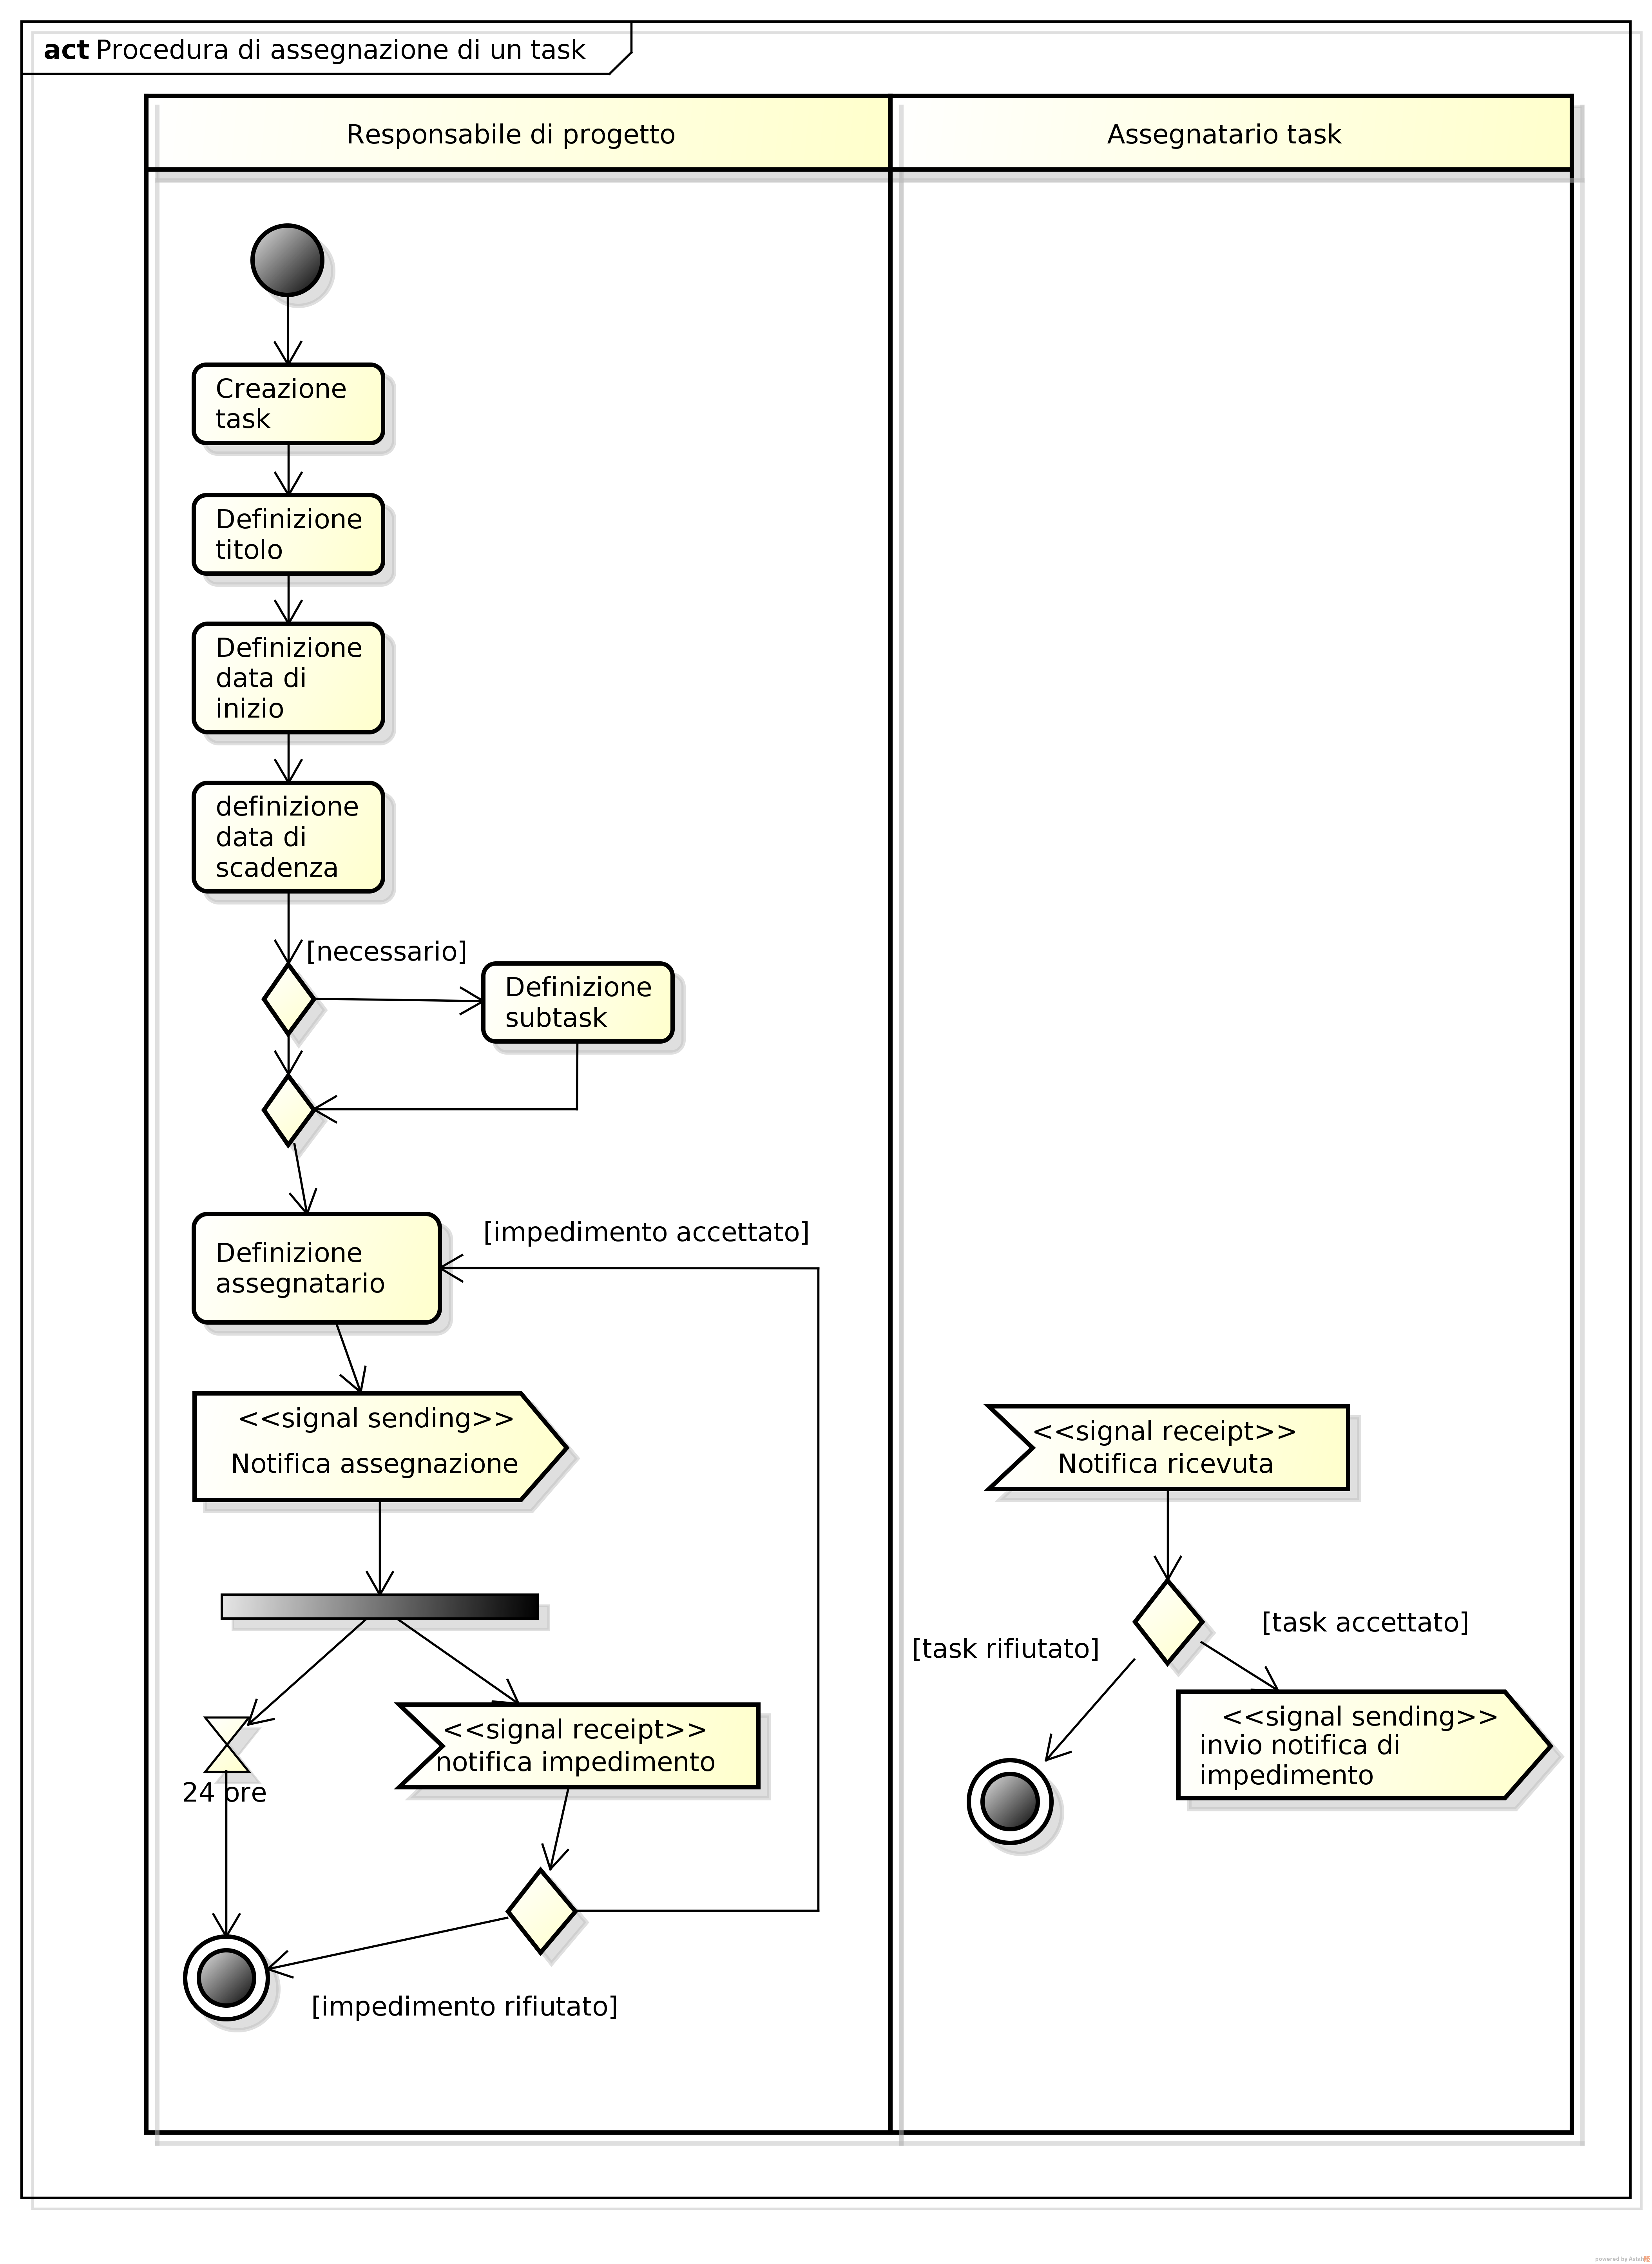
\includegraphics[scale=0.5]{png/Procedura di assegnazione di un task.png}
\captionsetup{labelfont=bf}
\caption{Diagramma di attività - Procedura di assegnazione di un task}

\end{figure}

\paragraph{Svolgimento di un task}
Il membro assegnatario del \textit{task}\G, ricevuta la notifica e non avendo alcun impedimento, dovrà procedere secondo le seguenti direttive:
\begin{itemize}
\item Se il \textit{task}\G\ ricevuto ha una scadenza più immediata rispetto a quello su cui sta lavorando, dovrà sospendere lo svolgimento di quest'ultimo, metterlo in coda e dedicarsi al \textit{task}\G\ appena notificato;
\item Se, dopo aver iniziato lo svolgimento del \textit{task}\G, si riceve la notifica di uno nuovo con scadenza più immediata si procederà come riportato nel punto precedente;
\item Se si dovesse superare la data di scadenza prevista, si dovrà impostare il tag "Delay" dal sistema di Teamwork\G.\\
Questa situazione si può verificare se:
\begin{itemize}
\item Il tempo assegnato dal \textit{Responsabile di progetto} non era sufficiente al completamento del \textit{task}\G;
\item Il \textit{task}\G\ in ritardo sta alle dipendenze di un altro non ancora terminato;
\item L'assegnatario ha rallentamenti esterni non resi noti al \textit{Responsabile di Progetto};
\item Il committente non ha a disposizione tutte le conoscenze necessarie al corretto svolgimento del \textit{task}\G.\\
\'E compito del \textit{Responsabile di Progetto} fare in modo che i primi due casi non si verifichino.
\end{itemize}
\item Al completamento del lavoro l'assegnatario dovrà spuntare il \textit{task}\G\ dalla lista presente su Teamwork\G;
\item Proseguire con lo svolgimento dei \textit{task}\G\ rimanenti seguendo la procedura dal suo inizio.
\end{itemize}

\paragraph{Rilevazione dei rischi}
Sarà compito del \textit{Responsabile di Progetto} individuare i rischi trovati nel \textit{Piano di Progetto v1.0.0}.\\
Questa attività necessita di un continuo monitoraggio, in quanto è plausibile che insorgano nuovi rischi in seguito a quelli rilevati nella fase preliminare. In tal caso il \textit{Responsabile di Progetto} dovrà agire come segue:
\begin{itemize}
\item Registrare il resoconto effettivo dei rischi nel \textit{Piano di Progetto v1.0.0};
\item Pianificare per gestire i nuovo rischi;
\item Aggiornare le metodologie per far fronte alla nuova pianificazione;
\item Monitorare i nuovo rischi riscontrati durante lo sviluppo del progetto. 
\end{itemize}

\paragraph{Ruoli di Progetto}
Ogni componente del gruppo \textit{Stark Labs} dovrà ricoprire almeno una volta ciascuno dei ruoli necessari allo sviluppo del progetto.\\
Vengono ora presentate le diverse cariche, delineando per ciascuna le mansioni e le responsabilità.

\subparagraph{Responsabile di Progetto} Il \textit{Responsabile di Progetto} rappresenta il \textit{team}\G\ e il progetto verso il committente e il proponente; accentra le responsabilità di scelta e approvazione.\\
Detiene le seguenti responsabilità:
\begin{itemize}
\item Pianificazione e coordinamento delle attività;
\item Gestione e controllo delle risorse;
\item Analisi e gestione dei rischi;
\item Approvazione dei documenti;
\item assicurarsi che tutte le attività svolte siano conformi alle \textit{Norme di Progetto
v1.0.0} e rispettino la pianificazione effettuata nel \textit{Piano di Progetto v1.0.0} .
\end{itemize}  

\subparagraph{Amministratore di Progetto} L' \textit{Amministratore di Progetto} deve svolgere i seguenti compiti:
\begin{itemize}
\item Assicurarsi che tutte le risorse siano presenti e operanti; 
\item Deve garantire un'infrastruttura funzionale;
\item Fornire procedure che servono a garantire la qualità del prodotto uscente da un
determinato compito.
\end{itemize}

\subparagraph{Analista} L' \textit{Analista} deve:
\begin{itemize}
\item Tradurre il bisogno del cliente in una specifica utile a trovare una soluzione;
\item Comprendere la complessità del problema;
\item Capire il dominio nel quale lavora il cliente;
\item Analizzare il dominio applicativo e le specifiche per poi produrre i documenti di analisi.
\end{itemize}
\subsubsection{Norme}

\subparagraph{Progettista} Il \textit{Progettista} ha il compito di:
\begin{itemize}
\item Individuare la tecnologia più idonea per risolvere il problema indicato dall' \textit{Analista};
\item Descrivere il funzionamento interno del sistema a diversi livelli di dettaglio;
\item Produrre una soluzione comprensibile e attuabile. 
\end{itemize}

\subparagraph{Programmatore} Il \textit{Programmatore} ha responsabilità sulle attività di codifica perciò deve:
\begin{itemize}
\item Scrivere codice documentato, versionato e manutenibile;
\item Implementare le soluzioni descritte dal \textit{Progettista};
\item Implementare i test sul codice prodotto. 
\end{itemize}

\subparagraph{Verificatore} Il \textit{Verificatore} è il responsabile delle attività di verifica, ha quindi i seguenti compiti:
\begin{itemize}
\item Controllare che vengano rispettate le norme di progetto;
\item Assicurarsi la conformità di ogni stadio del ciclo di vita del prodotto.
\end{itemize}
\subparagraph{Interne}
\subparagraph{Esterne}

\paragraph{Comunicazioni}
\subparagraph{Comunicazioni interne}
\subparagraph{Comunicazioni esterne}

\paragraph{Composizione email}
\subparagraph{Mittente}
\subparagraph{Destinatario}
\subparagraph{Corpo}
\subparagraph{Allegati}

\paragraph{Gestione ticket e milestones}
\subparagraph{Creazione e gestione dei ticket}
\subparagraph{Creazione delle milestone}
\subparagraph{Esecuzione dei compiti}
\subparagraph{Chiusura della milestone}

\subsubsection{Norme generali}
\paragraph{Ambiente di sviluppo}
\paragraph{Ruoli di progetto}
\subparagraph{Responsabile di progetto}
\subparagraph{Amministratore}
\subparagraph{Analista}
\subparagraph{Progettista}
\subparagraph{Verificatore}
\subparagraph{Programmatore}

\paragraph{Struttura del repository}
\subparagraph{Repository per la documentazione}
\subparagraph{Repository per il codice}
\subparagraph{Norme sull'utilizzo del servizio}

\subsubsection{Strumenti}

\paragraph{Sistema operativo}
\paragraph{Coordinamento}
\subparagraph{Teamwork?}
\subparagraph{Dropbox}
\subparagraph{Repository GIT}


\paragraph{Ambiente documentale}

\subparagraph{Stesura documenti}
\subparagraph{Script}

\paragraph{Pianificazione delle attività}

\paragraph{Diagrammi UML}
